\documentclass[11pt,a4paper]{article}
\usepackage[utf8]{inputenc}
\usepackage[T1]{fontenc}
\usepackage[ngerman]{babel}
\usepackage{lmodern,microtype}
\usepackage[left=22mm,right=22mm,top=24mm,bottom=22mm]{geometry}
\usepackage{graphicx,float,booktabs,tabularx,array,titlesec}
\usepackage{xcolor}
\usepackage[numbers,sort&compress]{natbib}
\usepackage{caption}
\usepackage{fancyhdr}
\usepackage[hidelinks]{hyperref}
\usepackage{xurl}

\newcommand{\KonzeptStand}{11. November 2026}

\hypersetup{pdftitle={CardHub -- Projektkonzeption},pdfauthor={CardHub-Projektteam}}
\setlength{\parindent}{0pt}
\setlength{\parskip}{5pt}
\setlength{\tabcolsep}{4pt}
\renewcommand{\arraystretch}{1.14}
\captionsetup{font=footnotesize,labelfont=bf,skip=5pt}
\setlength{\textfloatsep}{9pt}
\setlength{\intextsep}{8pt}
\setlength{\headheight}{14pt}
\pagestyle{fancy}
\fancyhf{}
\fancyhead[L]{\small CardHub}
\fancyhead[R]{\small Projektkonzeption}
\fancyfoot[C]{\thepage}
\renewcommand{\headrulewidth}{0.3pt}
\emergencystretch=2em
\titleformat{\section}{\normalfont\fontsize{15}{17.5}\bfseries}{\thesection.}{0.5em}{}
\titleformat{\subsection}{\normalfont\fontsize{11.9}{13.3}\bfseries}{\thesubsection}{0.5em}{}
\titlespacing*{\section}{0pt}{0pt}{9pt}
\titlespacing*{\subsection}{0pt}{7pt}{5pt}
\newif\ifmockups
\mockupstrue % Auf \mockupsfalse setzen, um den Anhang auszublenden.
\begin{document}
\begin{titlepage}
Technische Hochschule Mittelhessen\\
Fachbereich MNI\\[8mm]
Mobile Software Engineering\\
Wintersemester 2026/27
\vspace{29mm}
\begin{center}
{\Huge\bfseries CardHub\par}
\vspace{6mm}
{\LARGE Projektkonzeption\par}
\vspace{8mm}
{\large Mobile Anwendung zur Verwaltung\\von Pokémon-Sammelkarten\par}
\end{center}
\vfill
\textbf{Projektteam}\\[3mm]
\begin{tabular}{@{}ll@{}}
Louis Bieber & Ergänzen ????\\
Jerome-Pascal Habanz & 5321331\\
Rico Marco Libesch & 5324095\\
Mert Ali Özmeral & 5319592
\end{tabular}
\vspace{10mm}

\textbf{Dozent}\\Daniel Vogel
\vspace{8mm}

Stand: \KonzeptStand
\end{titlepage}
% Optional: Inhaltsverzeichnis als zusätzliche Vorseite.
% \tableofcontents\clearpage
\setcounter{page}{1}
\fontsize{10.8}{13.2}\selectfont
\section{Projektbeschreibung, Motivation und Zielgruppe}

\subsection{Ausgangssituation und Projektidee}
Mit einer wachsenden Pokémon-Kartensammlung wird es schwieriger, den Bestand im Blick zu behalten. Sammler möchten wissen, welche Karten sie besitzen, welche Exemplare fehlen und wie oft eine Karte vorhanden ist. Investmentorientierte Nutzer interessieren sich zusätzlich für Marktpreise und Wertentwicklung.

Vergleichbare Anwendungen sind bereits vorhanden. Nach Einschätzung des Projektteams sind viele davon unübersichtlich, wirken veraltet und bieten teure Abomodelle. Daraus entsteht die Motivation, eine Alternative mit einer zeitgemäßen und klar strukturierten Oberfläche zu entwickeln. CardHub verbindet Sammlungsverwaltung und Marktübersicht. Nutzer können Karten suchen, per Kamera erfassen und ihrer Sammlung hinzufügen. Einträge enthalten Anzahl, Kartendaten und verfügbare Preise. Die App ist für Android und iOS geplant und richtet sich an den deutschsprachigen Markt.

\subsection{Motivation und langfristige Vision}
Die Projektidee entstand aus dem eigenen Interesse des Teams an Pokémon-Karten. CardHub soll Erfassung und Verwaltung vereinfachen und Sammlung, Kartendetails und Marktwerte an einem Ort zugänglich machen.

Ein weiteres Ziel ist eine umfassende Übersicht über die Marktentwicklung verschiedener Karten. Nutzer sollen Marktwerte vergleichen und Veränderungen ihres Sammlungswerts nachvollziehen können. Langfristig zeigen Preisverläufe die Entwicklung einzelner Karten. So unterstützt CardHub das Sammeln als Hobby und die Beobachtung von Karten als Investment.

Das Endprodukt umfasst Pokédex, Sammlung, Tausch, Freunde und Profil. Nutzer sollen freigegebene Sammlungen ansehen und Tauschvorschläge austauschen können. Freundesfunktionen, Kartentausch, Gegenangebote, Tauschhistorie, Wunschlisten, Set-Fortschritt und das Erfassen mehrerer Karten in einem Durchgang folgen nach dem MVP.

\subsection{Zielgruppe und Folgen für die Bedienung}
Die primäre Zielgruppe sind deutschsprachige Erwachsene von 18 bis 40 Jahren mit einer physischen Pokémon-Kartensammlung. Die Altersspanne und die folgenden Merkmale sind Planungsannahmen für das Konzept. Hobby-Sammler suchen Überblick und Vollständigkeit. Investmentorientierte Nutzer verfolgen Marktpreise und Wertentwicklung. Deshalb trennt die Oberfläche Bestandsverwaltung und Marktinformationen klar.

Grundlegende Smartphone-Kenntnisse werden vorausgesetzt. Spielregeln und technisches Fachwissen sind nicht erforderlich. Bild, Name, Set und Nummer erleichtern die Zuordnung. Benötigt werden ein Android-Smartphone oder iPhone mit Kamera und für Sammlungsänderungen Internet. Zusätzliche Hardware ist nicht vorgesehen.

Das Konzept geht von sammelinteressierten, ordnungsorientierten und preisbewussten Nutzern aus. Daraus folgen eine übersichtliche Sammlung, eine schnelle Suche und einfache Mengenänderungen.

Unterschiede bei Sehvermögen und Treffsicherheit werden berücksichtigt. Dafür sind anpassbare Schriftgrößen, klare Kontraste und große Bedienelemente vorgesehen. Hinweise werden durch Text und nicht allein durch Farbe vermittelt.

Vorgesehene Situationen sind wiederholte Scans nach dem Öffnen von Boostern, kurze Preischecks unter Zeitdruck und das Ordnen in der Freizeit. Scan und Suche bleiben direkt erreichbar. Nach einem Scan kann die nächste Karte erfasst werden.

Die App soll neben Ausbildung, Studium, Beruf oder Familienaufgaben nutzbar sein. Einkommen und Familienstand werden nicht eingegrenzt. Unterschiedliche Budgets und begrenzte Freizeit sprechen für kurze, unterbrechbare Abläufe und klar bezeichnete Preise mit Datenstand.


\clearpage
\section{Anforderungen und Umfang des MVP}

Das Minimum Viable Product deckt den Kernablauf vollständig ab: Eine angemeldete Person erfasst eine Karte, bestätigt die Zuordnung und findet sie anschließend in ihrer Sammlung wieder. Der Kursumfang umfasst Anmeldung, Katalog, Kartenerkennung, manuelle Eingabe, Sammlung und Preisübersicht. Die folgenden Anforderungen legen diesen Umfang fest.

\subsection{Funktionale Anforderungen}
\begin{table}[H]
\centering
\small
\begin{tabularx}{\linewidth}{@{}>{\hsize=0.56\hsize\linewidth=\hsize\raggedright\arraybackslash}X >{\hsize=1.44\hsize\linewidth=\hsize\raggedright\arraybackslash}X@{}}
\toprule
\textbf{Funktion} & \textbf{Umfang im MVP} \\
\midrule
Konto und Sitzung & Registrieren, anmelden und abmelden. Persönliche Sammlungsdaten sind nur nach Anmeldung zugänglich. \\
Kartenkatalog & Den gesamten deutschen TCGdex-Katalog durchsuchen. Nach Name oder Nummer suchen, nach Set oder Typ filtern und Details anzeigen. \\
Kameraerfassung & Kartenaufnahmen durch ein KI-Modell lokal auf dem Smartphone zuordnen. Ziel ist der gesamte deutsche TCGdex-Katalog. Mögliche Treffer zur Bestätigung anzeigen. Wird keine passende Karte erkannt, die manuelle Suche anbieten. \\
Manuelle Eingabe & Eine Karte nach Name oder Nummer suchen, auswählen und mit einer Anzahl übernehmen. Die Eingabe ist direkt und nach einem fehlgeschlagenen Scan möglich. \\
Sammlung verwalten & Eigene Karten anzeigen und filtern. Anzahl online erhöhen oder verringern und Einträge entfernen. \\
Preise und Gesamtwert & Verfügbare Euro-Richtwerte mit Datenstand anzeigen. Aus bewertbaren Einträgen einen geschätzten Gesamtwert berechnen. \\
\bottomrule
\end{tabularx}
\caption{Funktionaler Umfang des MVP. Eigene Darstellung.}
\end{table}
\subsection{Nichtfunktionale Anforderungen}
\begin{table}[H]
\centering
\small
\begin{tabularx}{\linewidth}{@{}>{\hsize=0.56\hsize\linewidth=\hsize\raggedright\arraybackslash}X >{\hsize=1.44\hsize\linewidth=\hsize\raggedright\arraybackslash}X@{}}
\toprule
\textbf{Qualitätsziel} & \textbf{Prüfbares Verhalten} \\
\midrule
Plattformen & Den Kernablauf auf mindestens einem Android-Gerät und einem iPhone prüfen. \\
Fehlertoleranz & Bei uneindeutiger Erkennung mehrere mögliche Treffer zur Auswahl anbieten. Der Nutzer kann falsche Vorschläge verwerfen und einen anderen Treffer wählen. Passt kein Vorschlag, ist die manuelle Suche verfügbar. \\
Datenschutz und Zugriff & Scanbilder nur vorübergehend im Arbeitsspeicher verarbeiten. Die App speichert sie nicht als Dateien und überträgt sie nicht an das Backend. Persönliche Sammlungsdaten sind nur für den angemeldeten Nutzer zugänglich. \\
Datenqualität & Keine negativen Mengen speichern. Fehlende Preise nicht als 0 Euro ausgeben. Änderungen erst nach Serverbestätigung als gespeichert anzeigen. \\
Wartbarkeit und Betrieb & Komponenten und Schnittstellen trennen. Den Backend-Start mit einer dokumentierten Compose-Konfiguration reproduzieren. \\
\bottomrule
\end{tabularx}
\caption{Aus den Anwendungsfällen abgeleitete Qualitätsanforderungen. Eigene Darstellung.}
\end{table}
\subsection{Abgrenzung und spätere Erweiterungen}
Freundesverwaltung, fremde Sammlungen, Tausch und Gegenangebote folgen nach dem MVP. Auch Profilbilder, Chat, Wunschliste, Preisalarme und Release-Kalender sind spätere Erweiterungen. Sammlungsänderungen erfordern im MVP eine Internetverbindung. Offline-Bearbeitung mit späterer Synchronisation ist ausgeschlossen. Die Kartenerkennung umfasst als Ziel den gesamten deutschen TCGdex-Katalog. Eine Begrenzung auf einzelne Sets oder einen Pilotbestand ist nicht vorgesehen.


\clearpage
\section{Akteure und Anwendungsfälle}

CardHub hat vier Akteure. Der \textbf{Gast} ist nicht angemeldet. Er legt ein Konto an oder meldet sich an. Der \textbf{Sammler} ist angemeldet und der primäre Akteur. Ein \textbf{Freund} ist ein Sammler mit bestätigter Freundschaft. Er tritt erst im Ausbau auf. Der \textbf{API-Aufrufer} ist ein technischer Akteur. Er startet regelmäßig den Import von Kartendaten und Preisen aus der TCGdex-API. Kamera und Erkennungsmodell gehören zur App und sind keine Akteure.

\begin{figure}[H]
\centering
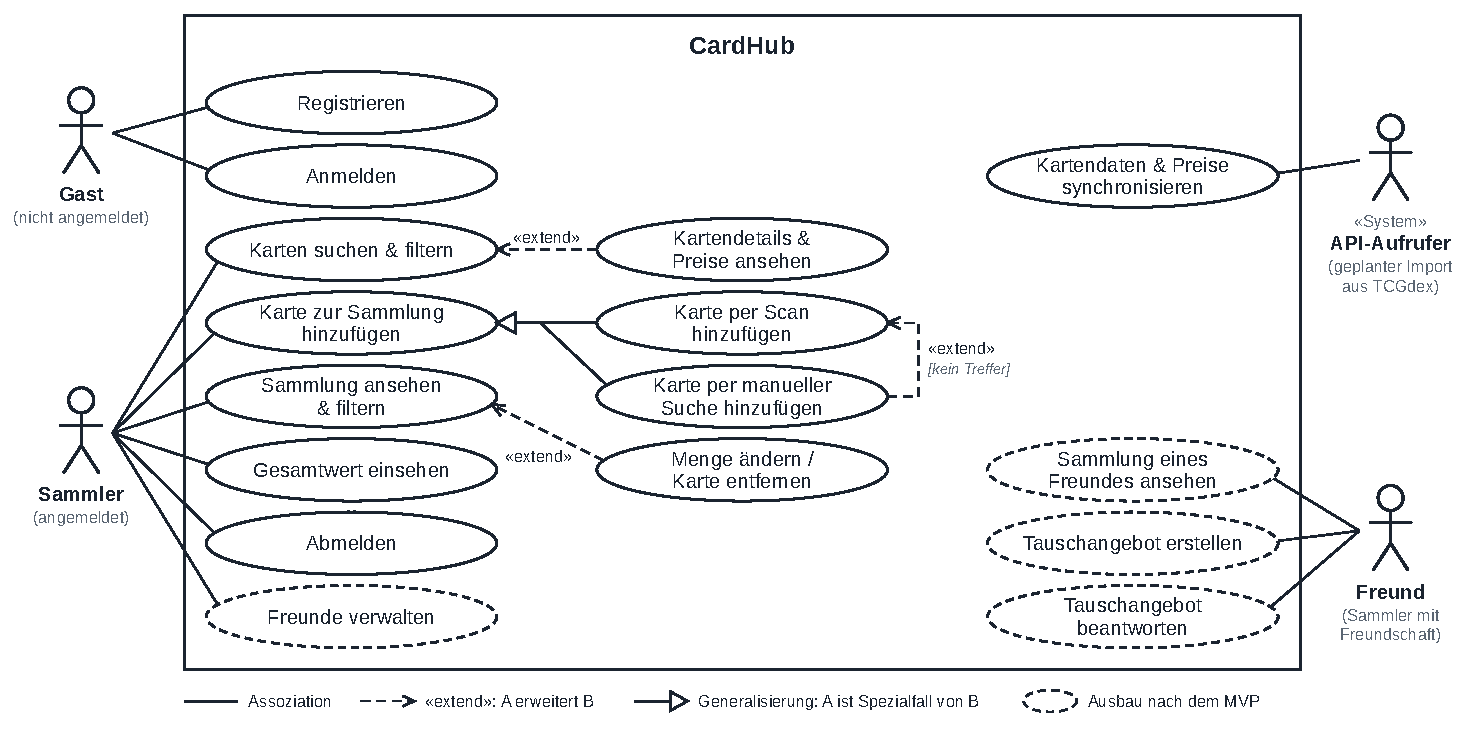
\includegraphics[width=\linewidth,height=8.2cm,keepaspectratio]{diagramme/usecases.pdf}
\caption{Use-Case-Diagramm für MVP und Ausbau. Eigene Darstellung.}
\label{fig:usecases}
\end{figure}
\subsection{Anwendungsfälle im Überblick}
Abbildung~\ref{fig:usecases} zeigt alle Anwendungsfälle. Nach der Anmeldung handelt der Gast als Sammler. Der Sammler sucht Karten im Katalog und filtert nach Set oder Typ. Kartendetails und Preise erweitern die Suche. Karten fügt er per Scan oder per manueller Suche hinzu. Beide Wege sind Spezialfälle von \emph{Karte zur Sammlung hinzufügen}. Die manuelle Suche erweitert den Scan, wenn kein Vorschlag passt. In der Sammlung ändert er Mengen oder entfernt Einträge. Der Gesamtwert summiert die Richtwerte.

Im Ausbau verwaltet der Sammler seine Freunde. Ein Freund sieht freigegebene Sammlungen und erstellt ein Tauschangebot. Der Empfänger nimmt es an, lehnt es ab oder stellt ein Gegenangebot.

\subsection{Hauptanwendungsfall: Karte per Scan hinzufügen}
\textbf{Vorbedingung:} Der Sammler ist angemeldet und hat die Kamera freigegeben. \textbf{Ablauf:} (1)~Der Sammler startet den Scanner und nimmt die Karte auf. (2)~Das lokale Modell ermittelt bis zu fünf Kandidaten. (3)~Der Sammler wählt den Treffer und legt die Anzahl fest. (4)~Die App sendet Karten-ID und Anzahl an das Backend. (5)~Nach der Bestätigung des Servers zeigt die App den Eintrag. \textbf{Alternativen:} Passt kein Kandidat, sucht der Sammler die Karte manuell. Bei einem Netzfehler bleibt die Auswahl erhalten. \textbf{Ergebnis:} Die Sammlung enthält die Karte mit positiver Anzahl.

\subsection{Folgerungen für Software-Design und Technologie-Stack}
Der Scan läuft auf dem Gerät. Die App braucht Kamera und lokales Modell auf Android und iOS. Die Sammlung ist geschützt. Ein zentrales Gateway prüft bei jeder Anfrage die Anmeldung. Katalog und Preise liefert ein Fremdsystem. Ein eigener Dienst importiert sie. Mengen und späterer Tausch verlangen konsistente Bestände. Dafür eignet sich eine relationale Datenbank mit Transaktionen.

\clearpage
\section{Systemarchitektur und Verantwortlichkeiten}

CardHub besteht aus einer mobilen Anwendung, einem API-Gateway und drei Backend-Diensten. Die vollständige Zielarchitektur ist in Anhang A dargestellt. Sie umfasst auch spätere Funktionen wie Freunde, Profile und Tausch.

Die mobile App stellt die Oberfläche bereit und verwaltet den Anmeldestatus. Die Kamera liefert das Bild für die lokale Kartenerkennung. Das KI-Modell läuft direkt auf dem Smartphone und gibt mögliche Treffer zurück. Der Nutzer bestätigt die passende Karte oder sucht sie manuell. Das Modell wird außerhalb der App trainiert. Modell und Kartenzuordnung werden gemeinsam versioniert und in der App bereitgestellt.

Die App sendet Backend-Anfragen ausschließlich an das API-Gateway. Es prüft das Zugangstoken, begrenzt die Anzahl der Anfragen und leitet sie an den zuständigen Dienst weiter. Die Go-Dienste kommunizieren intern über gRPC.

Der Identitätsdienst verwaltet Konten, Anmeldung und später Profile sowie Freundschaften. Der Katalogdienst stellt Karten, Sets, Suche und Preise bereit. Er gleicht Karten- und Marktdaten mit externen Quellen ab. Der Bestandsdienst verwaltet Sammlungen und Mengen. Für Kartendaten fragt er den Katalogdienst ab. Später verarbeitet er auch Tauschangebote und Gegenangebote.

Jeder Dienst verwaltet eine eigene logische Datenbank innerhalb einer PostgreSQL-Instanz. Die App greift nicht direkt auf die Datenbanken zu. Der Identitätsdienst nutzt später einen Objektspeicher für Profilbilder. Scanbilder werden nur vorübergehend im Arbeitsspeicher verarbeitet. Sie werden weder dauerhaft gespeichert noch an das Backend übertragen.

\section{Systemarchitektur und Verantwortlichkeiten}

CardHub besteht aus einer mobilen Anwendung, einem API-Gateway und drei Backend-Diensten. Die vollständige Zielarchitektur ist in Anhang A dargestellt. Sie umfasst auch spätere Funktionen wie Freunde, Profile und Tausch.

Die mobile App stellt die Oberfläche bereit und verwaltet den Anmeldestatus. Die Kamera liefert das Bild für die lokale Kartenerkennung. Das KI-Modell läuft direkt auf dem Smartphone und gibt mögliche Treffer zurück. Der Nutzer bestätigt die passende Karte oder sucht sie manuell. Das Modell wird außerhalb der App trainiert. Modell und Kartenzuordnung werden gemeinsam versioniert und in der App bereitgestellt.

Die App sendet Backend-Anfragen ausschließlich an das API-Gateway. Es prüft das Zugangstoken, begrenzt die Anzahl der Anfragen und leitet sie an den zuständigen Dienst weiter. Die Go-Dienste kommunizieren intern über gRPC.

Der Identitätsdienst verwaltet Konten, Anmeldung und später Profile sowie Freundschaften. Der Katalogdienst stellt Karten, Sets, Suche und Preise bereit. Er gleicht Karten- und Marktdaten mit externen Quellen ab. Der Bestandsdienst verwaltet Sammlungen und Mengen. Für Kartendaten fragt er den Katalogdienst ab. Später verarbeitet er auch Tauschangebote und Gegenangebote.

Jeder Dienst verwaltet eine eigene logische Datenbank innerhalb einer PostgreSQL-Instanz. Die App greift nicht direkt auf die Datenbanken zu. Der Identitätsdienst nutzt später einen Objektspeicher für Profilbilder. Scanbilder werden nur vorübergehend im Arbeitsspeicher verarbeitet. Sie werden weder dauerhaft gespeichert noch an das Backend übertragen.


\clearpage
\section{Technologieevaluation und Auswahl}

Die Auswahl richtet sich nach Android- und iOS-Unterstützung, Kamera- und ML-Anbindung, Datenkonsistenz und Aufwand im Kurs. Festgelegt sind Kotlin mit Compose Multiplatform, Go-Dienste, gRPC, PostgreSQL und Docker Compose. Für die Kartenerkennung sind PyTorch und ONNX vorgesehen. Die Evaluation begründet diese Auswahl gegenüber den betrachteten Alternativen.

\subsection{Mobile Anwendung}
\begin{table}[H]
\centering
\small
\begin{tabularx}{\linewidth}{@{}>{\hsize=0.75\hsize\linewidth=\hsize\raggedright\arraybackslash}X >{\hsize=1.17\hsize\linewidth=\hsize\raggedright\arraybackslash}X >{\hsize=1.08\hsize\linewidth=\hsize\raggedright\arraybackslash}X@{}}
\toprule
\textbf{Alternative} & \textbf{Vorteil} & \textbf{Nachteil im Projekt} \\
\midrule
Native Oberflächen & Direkter Zugriff auf Plattformfunktionen und jeweilige UI-Werkzeuge. & Oberflächen für Android und iOS müssen getrennt umgesetzt werden. \\
Flutter & Gemeinsame Oberfläche und Anwendungslogik für beide Plattformen. & Dart kommt als weitere Sprache hinzu. Kamera und ML benötigen Plattformanbindung. \\
Kotlin und Compose Multiplatform & Gemeinsame Logik und Oberfläche; Kotlin passt zum bisherigen Projektvorschlag. & Kamera, Modell und sichere Ablage brauchen teilweise plattformspezifischen Code. \\
\bottomrule
\end{tabularx}
\caption{Projektbezogener Vergleich auf Grundlage der Framework-Dokumentationen. Eigene Bewertung. \cite{kmp,flutter}}
\end{table}
Die App wird mit Kotlin Multiplatform und Compose Multiplatform umgesetzt. Damit lassen sich Anwendungslogik und große Teile der Oberfläche für Android und iOS teilen. Die gemeinsame UI verwendet auf iOS nicht automatisch native SwiftUI-Bedienelemente. Kamera, Modell und sichere Ablage werden über plattformspezifische Anbindungen eingebunden und auf beiden Plattformen geprüft. Flutter bleibt eine mögliche Alternative; die gemeinsame Kotlin-Oberfläche ist für CardHub verbindlich gewählt. \cite{kmp}

\subsection{Backend, Daten und Bereitstellung}
\begin{table}[H]
\centering
\small
\begin{tabularx}{\linewidth}{@{}>{\hsize=0.63\hsize\linewidth=\hsize\raggedright\arraybackslash}X >{\hsize=0.8699999999999999\hsize\linewidth=\hsize\raggedright\arraybackslash}X >{\hsize=1.5\hsize\linewidth=\hsize\raggedright\arraybackslash}X@{}}
\toprule
\textbf{Bereich} & \textbf{Auswahl / Alternative} & \textbf{Begründung für CardHub} \\
\midrule
Backend & Go-Dienste / Monolith / Supabase & Ein Monolith wäre einfacher zu betreiben. Supabase bündelt Standardfunktionen. Festgelegt sind eigene Go-Dienste mit drei Fachgrenzen; die Aufteilung trennt Konten, Katalog und Bestände. \\
Kommunikation & REST/JSON außen; gRPC innen / durchgehend REST & JSON hält den mobilen Zugriff einfach. Protocol Buffers beschreiben interne Verträge und ermöglichen generierte Schnittstellen. \\
Datenbank & PostgreSQL / MongoDB & Bestände, Konten und Angebote sind relational. SQL-Regeln und Transaktionen passen zu Mengen und gemeinsamen Bestandsänderungen. \\
Kartendaten & TCGdex / Pokémon TCG API & TCGdex bietet deutsche Kartendaten und Cardmarket-Richtwerte. Verfügbarkeit und Zuordnung werden geprüft. Die ältere Pokémon TCG API ist als veraltet gekennzeichnet. \\
Bilder und Betrieb & SeaweedFS; Compose / Dateisystem; manueller Start & SeaweedFS ist für Profilbilder im Ausbau vorgesehen. Seine S3-Schnittstelle trennt die Dateiablage vom Dienst. Compose beschreibt Dienste, Netzwerke und Volumes für einen gemeinsamen Start. \\
\bottomrule
\end{tabularx}
\caption{Technologieauswahl und Begründung. Eigene Bewertung auf Grundlage der offiziellen Dokumentationen. \cite{grpc,postgres,tcgdex,preise,alteapi,seaweed,compose}}
\end{table}

\clearpage
\section{Kartenerkennung und Datenhaltung}

\subsection{Hybride Kartenerkennung und mobile Ausführung}
Die Kartenerkennung verbindet Bildvergleich und Texterkennung. OpenCV erkennt die Kartenkontur und richtet das Bild aus. DINOv2-small erzeugt einen Merkmalsvektor des Bildes. Dieser wird mit gespeicherten Referenzvektoren verglichen. Eine ergänzende Texterkennung liest Kartenname und Sammlernummer. Ein Ranking verbindet Bildtreffer und deutsche TCGdex-Metadaten. So können auch Karten ohne Referenzbild über Text in die Vorschlagsliste gelangen. \cite{dinov2}

Python und PyTorch bilden die Trainingsgrundlage. Der Code unterstützt die Anpassung des vortrainierten DINOv2-Modells durch kontrastives Fine-Tuning. Als Trainingsquelle sind Referenzbilder oder gelabelte Fotos vorgesehen. Validierungs- und Testfotos werden nach Karten-ID getrennt. Dieser Ansatz passt zum Bildvergleich und nutzt ein vorhandenes Modell. Reine OCR und reine Bildsuche werden als Vergleichsvarianten untersucht.

Der Export erzeugt ein ONNX-Modell mit Opset 18. Zum versionierten Paket gehören Referenzvektoren, Kartenkatalog, Ranking-Gewichte und Angaben zur Bildvorbereitung. Der Python-Code prüft Modell und Export auf übereinstimmende Ausgaben. Für die mobile Modellausführung ist ONNX Runtime vorgesehen. Die Anbindung an die Kotlin-App und der Vergleich auf Android und iOS sind noch umzusetzen. \cite{onnxmobile}

Im Python-Prototyp wird RapidOCR verwendet. Das OCR-Werkzeug für die mobile App bleibt offen. Die Oberfläche zeigt bis zu fünf Kandidaten zur Bestätigung. Ranking-Werte sind keine garantierten Wahrscheinlichkeiten. Bei unpassenden Treffern bleibt die manuelle Suche verfügbar. Zielumfang ist der gesamte deutsche TCGdex-Katalog.

\subsection{Datenmodell und Preisangaben}
\begin{table}[H]
\centering
\small
\begin{tabularx}{\linewidth}{@{}>{\hsize=0.5\hsize\linewidth=\hsize\raggedright\arraybackslash}X >{\hsize=1.5\hsize\linewidth=\hsize\raggedright\arraybackslash}X@{}}
\toprule
\textbf{Datenbereich} & \textbf{Zentrale Daten} \\
\midrule
Identity & Nutzer-ID, Kontodaten und erneuerbare Sitzungen; später Freundschaft und Profilbild-Metadaten. \\
Catalog & Karten-ID, Sprache, Set, Nummer und Variante. Preisstände enthalten Quelle, Währung, Wert und Aktualisierungszeit. \\
Inventory & Nutzer-ID, Karten-ID, Sprache, Variante und Menge. Später Angebot, Angebotspositionen und Statusänderungen. \\
\bottomrule
\end{tabularx}
\caption{Fachliches Datenmodell. Eigene Darstellung.}
\end{table}
Die Datenbanken werden nicht durch dienstübergreifende Fremdschlüssel gekoppelt. Karten- und Nutzer-IDs sind Referenzen, die über die zuständigen Dienste geprüft werden. Für dieselbe Kombination aus Nutzer, Karte, Sprache und Variante gibt es einen zusammengefassten Bestand. Preisstände bleiben vom Besitz getrennt: Eine Preisänderung ändert keine Kartenmenge.

TCGdex dokumentiert fehlende Preise und mögliche Fehlzuordnungen zwischen Varianten. Die App nennt deshalb Quelle und Datenstand. Nicht bewertbare Einträge werden gesondert gezählt. Ein Durchschnitt für einen Zeitraum ist kein vollständiger Preisverlauf. Für eigene Verlaufsgrafiken müssten über längere Zeit passende Preisstände gespeichert werden. Der geschätzte Gesamtwert ist die Summe aus Anzahl mal verfügbarem Richtwert je Eintrag. Zustand und konkrete Verkaufssituation können davon abweichen. \cite{preise,preisfaq}

Die Bildanalyse soll lokal auf dem Smartphone erfolgen. Sammlungsänderungen werden im MVP nur mit Internetverbindung gespeichert. Der Server bleibt die verbindliche Quelle des Bestands. Nach einem Netzfehler bleibt die Auswahl für einen erneuten Versuch erhalten; eine Offline-Synchronisation wird nicht umgesetzt.


\clearpage
\section{Konsistenz, UI-Konzept und Umsetzung}

\subsection{Sicherheit und geplanter Tausch}
Für die Anmeldung sind kurzlebige JWT-Zugangstoken und erneuerbare Sitzungen vorgesehen. Das Gateway prüft die Token. Jeder Dienst prüft zusätzlich die Berechtigung für die betroffene Ressource. Nutzer-IDs aus frei änderbaren Eingaben reichen dafür nicht aus. Passwörter werden mit Argon2id gehasht. Abmelden widerruft die erneuerbare Sitzung. Zugangsdaten werden geschützt auf dem Gerät abgelegt. Nur der Reverse Proxy ist öffentlich erreichbar; Datenbanken und interne Dienste bleiben im privaten Netz.

Sammlung und Tausch gehören zum Inventory Service. Beim späteren Annehmen eines Angebots werden Status und betroffene Bestände in einer Transaktion gesperrt und geprüft. Alle Mengenänderungen werden gemeinsam gespeichert oder vollständig verworfen. Bereits abgeschlossene Angebote dürfen keine zweite Änderung auslösen. Karten werden bei offenen Angeboten zunächst nicht reserviert; ihre Verfügbarkeit wird beim Annehmen erneut geprüft. \cite{postgres}

\begin{figure}[H]
\centering
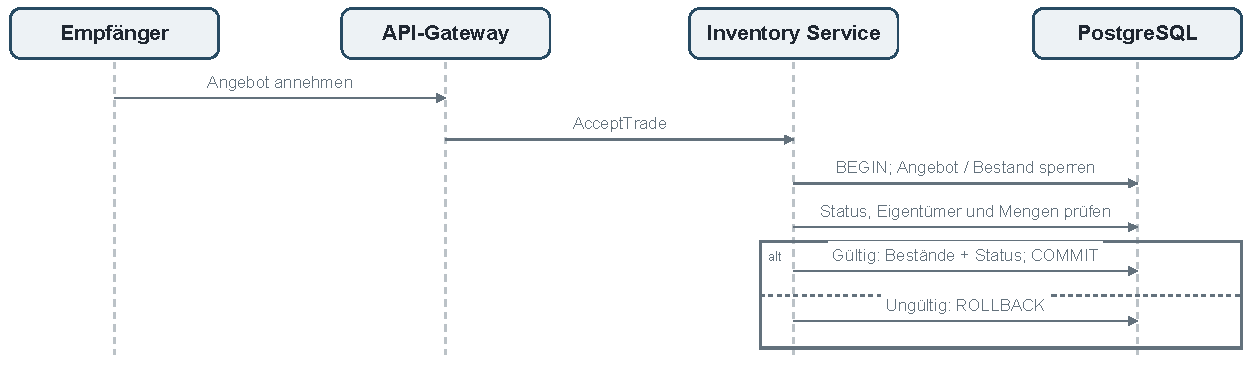
\includegraphics[width=\linewidth,height=4.7cm,keepaspectratio]{diagramme/tausch.pdf}
\caption{Annahme eines Tauschangebots im späteren Ausbau. Eigene Darstellung.}
\label{fig:tausch}
\end{figure}
\subsection{UI-Konzept und Mockup-Ablauf}
Die Zielnavigation umfasst Pokédex, Tausch, Sammlung, Freunde und Profil. Im MVP sind nur umgesetzte Bereiche aktiv. Die Sammlung bündelt Scan, manuelle Eingabe, Mengen und Wertübersicht. Kartenbilder werden stets durch Name, Set und Nummer ergänzt. Hinweise nennen eine konkrete Handlung. Das vorhandene Gestaltungskonzept orientiert sich an Apples Human Interface Guidelines; Android-Bedienmuster werden beim Geräteversuch mitgeprüft. \cite{apple}

Der Mockup-Anhang zeigt später den Weg Sammlung, Kamera, Trefferwahl, Mengenangabe und gespeicherter Eintrag. Ein zweiter Ablauf zeigt die manuelle Suche. Die Mockups stellen den geplanten Ablauf mit Beispieldaten dar. Sie sind kein Nachweis einer bereits abgeschlossenen Implementierung.

\subsection{Vorgehen und Qualitätssicherung}
Die Umsetzung beginnt mit der Anbindung des vorhandenen Erkennungsansatzes an die mobile App. Danach werden Backend-Grundlage und Anmeldung, Katalog und Preise sowie Sammlung und Scan integriert. Der MVP wird vor den sozialen Erweiterungen abgeschlossen. Schnittstellen und Abnahmekriterien werden dokumentiert. Änderungen am gemeinsamen Stand werden geprüft.

Die Abnahme prüft den Kernablauf auf Android und iOS. Dazu gehören Kameraverweigerung, falsche Treffer, Netzfehler, fehlende Preise und fremde Nutzer-IDs. Neue, bei der Entwicklung nicht genutzte Fotos dienen zur Messung von Top-1-, Top-3- und Top-5-Treffern sowie Antwortzeit und Speicherbedarf. Die bisherige Testauswahl belegt noch keine Erkennung des Gesamtkatalogs. Für den späteren Tausch werden parallele Annahmen und fehlende Karten geprüft. Der Backend-Start muss aus einem frischen Compose-Stand nachvollziehbar sein.



\clearpage
\addcontentsline{toc}{section}{Literatur}
\begingroup
\small
\bibliographystyle{unsrt}
\bibliography{quellen}
\endgroup
\clearpage
\appendix
% Dedicated full-page architecture diagram.
\newgeometry{left=10mm,right=10mm,top=8mm,bottom=10mm}
\thispagestyle{plain}
\section{Systemarchitektur}
\label{anh:architektur}
\begingroup
\setlength{\intextsep}{4pt}
\captionsetup{skip=3pt}
\begin{figure}[H]
\centering
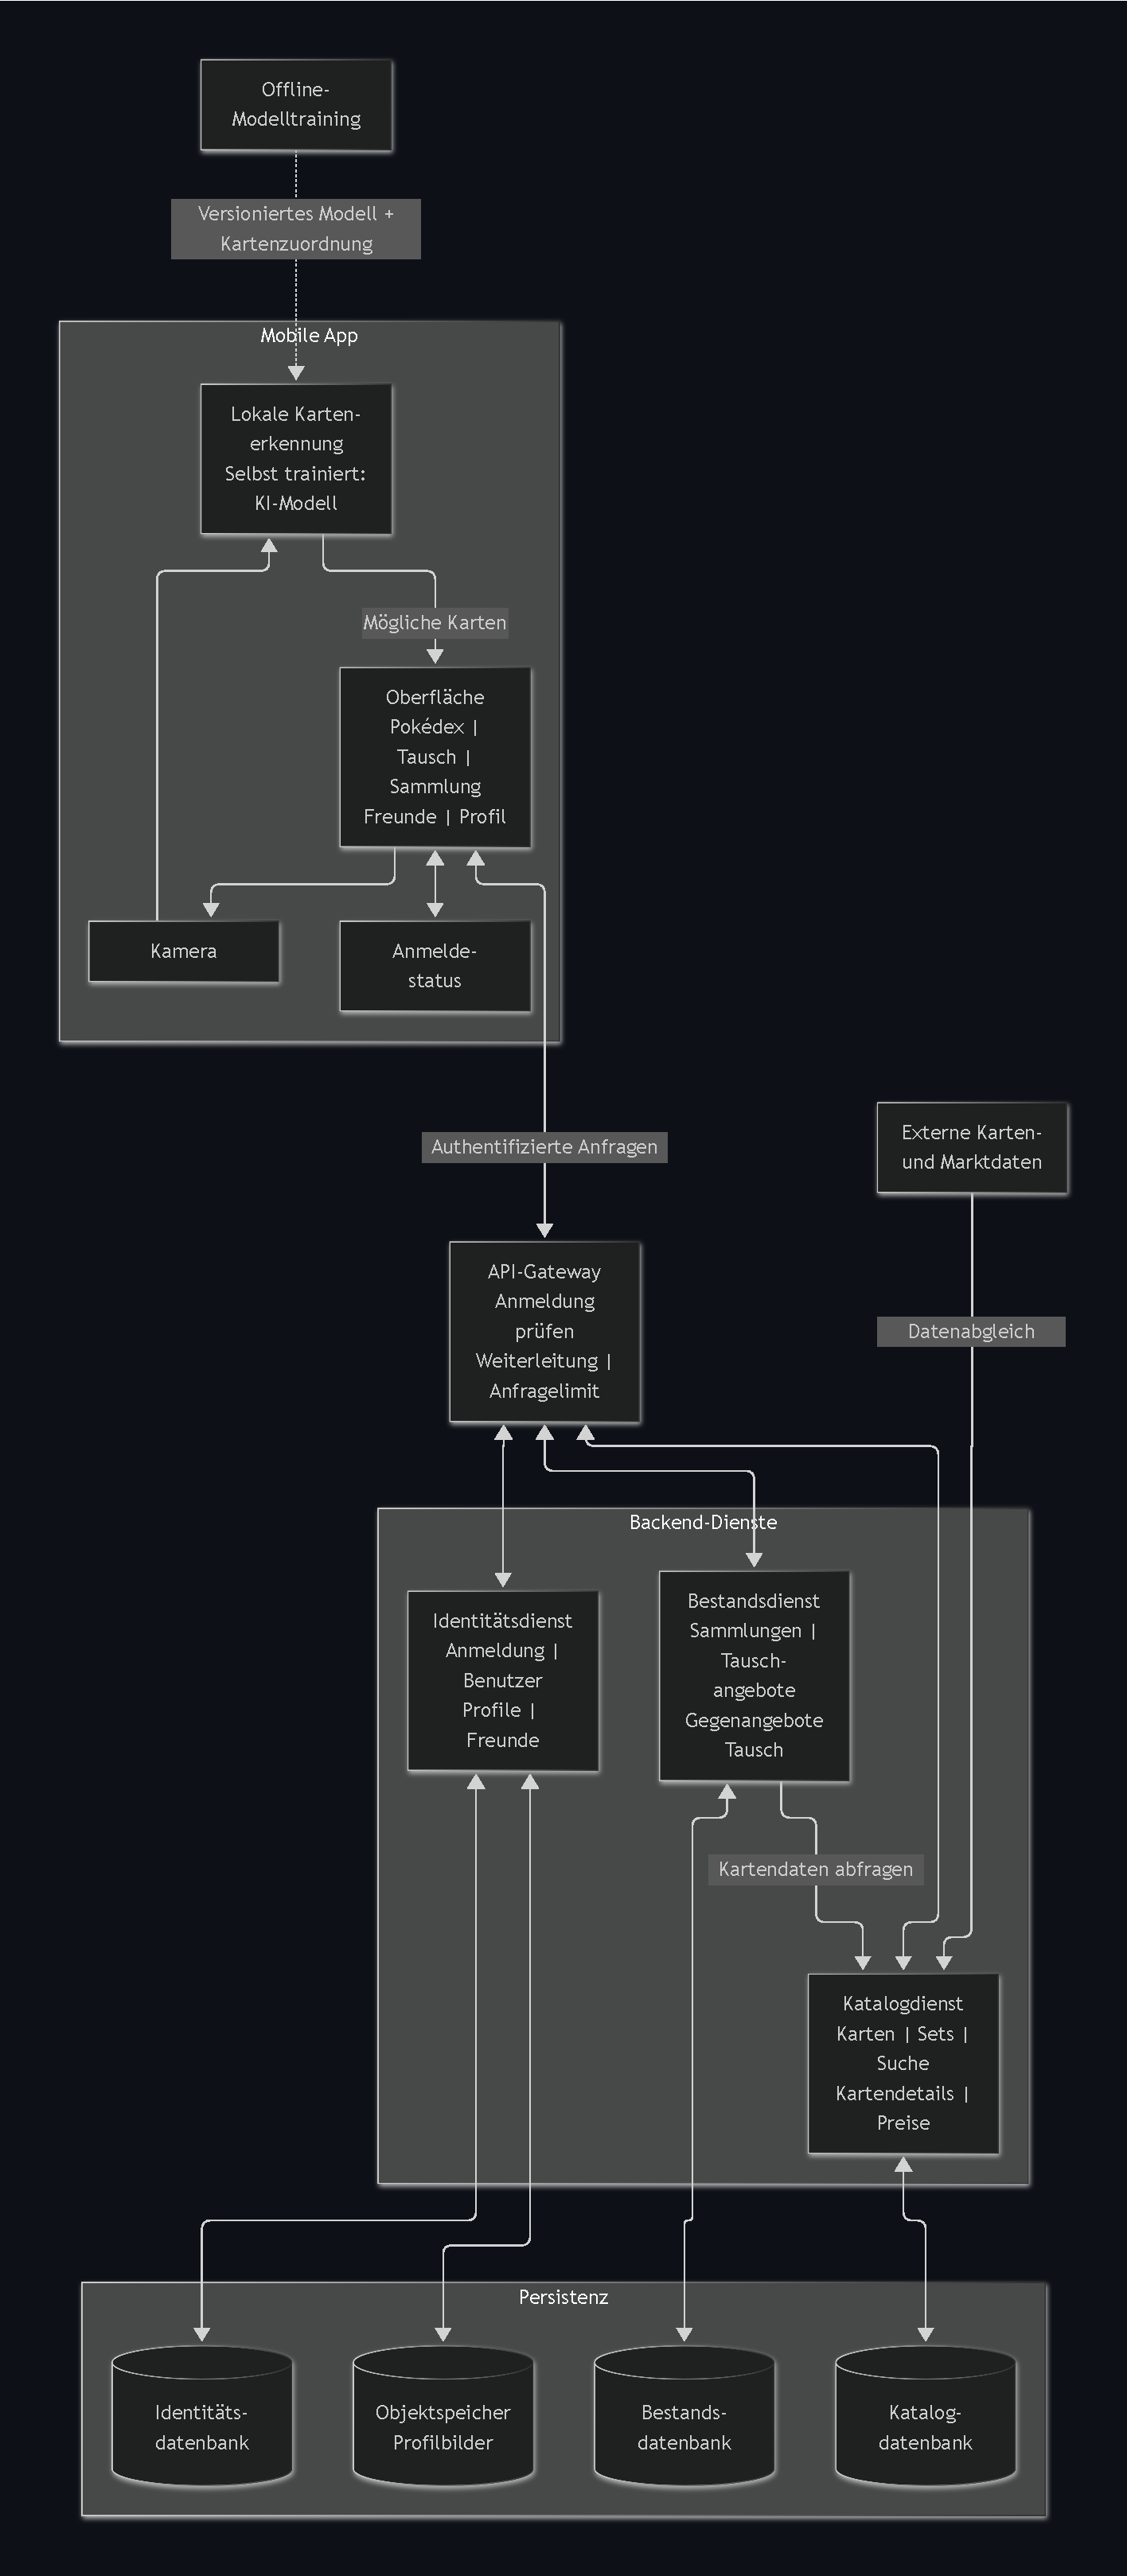
\includegraphics[width=\linewidth,height=\dimexpr\textheight-66pt\relax,keepaspectratio]{diagramme/architektur.pdf}
\caption{Vollständige Zielarchitektur von CardHub.}
\label{fig:architektur-gesamt}
\end{figure}
\endgroup
\restoregeometry

\ifmockups
\clearpage
%\section{UI-Mockups}
Die folgenden Ansichten werden vor der Abgabe durch die finalen Mockups ersetzt. Der Hauptablauf muss vom Start bis zum gespeicherten Sammlungseintrag visuell nachvollziehbar sein. Die manuelle Suche zeigt den alternativen Weg bei einem fehlgeschlagenen Scan.

\newcommand{\mockslot}[2]{%
\begin{minipage}[t]{0.47\linewidth}\centering
\IfFileExists{mockups/#1}{\includegraphics[width=0.96\linewidth,height=59mm,keepaspectratio]{mockups/#1}}{\fbox{\parbox[c][57mm][c]{0.88\linewidth}{\centering\small #2\\[4mm]\texttt{\detokenize{#1}}}}}\\[2mm]
{\small #2}
\end{minipage}}
\begin{figure}[H]\centering
\mockslot{01-sammlung.png}{1. Sammlung öffnen}\hfill
\mockslot{02-scanner.png}{2. Karte aufnehmen}\par\vspace{4mm}
\mockslot{03-treffer.png}{3. Treffer bestätigen}\hfill
\mockslot{04-menge.png}{4. Anzahl festlegen}\par\vspace{4mm}
\mockslot{05-gespeichert.png}{5. Gespeicherten Eintrag ansehen}\hfill
\mockslot{06-manuelle-suche.png}{Alternative: manuelle Suche}
\caption{Hauptablauf und manuelle Alternative. Eigene Darstellung. Die sichtbaren Felder sind Platzhalter für die finalen Mockups.}
\end{figure}

\fi
\end{document}
